\documentclass[reqno,10pt]{amsart}

%%%%%%%%%% Packages %%%%%%%%%%

\usepackage{amsmath,bbm,verbatim,wasysym,nicefrac,amssymb,braket}
%mathtools,appendix,soul,ulem,slashed,upgreek
\usepackage[protrusion=true, babel=true]{microtype}
\usepackage[english]{babel}
\usepackage[widespace]{fourier}
\usepackage[backrefs]{amsrefs}
\usepackage[margin=1in]{geometry}
\usepackage[onehalfspacing]{setspace}
\usepackage[pdfusetitle,pagebackref]{hyperref}
\numberwithin{equation}{section}                % must be called before cleveref
\usepackage[nameinlink,noabbrev]{cleveref}
\expandafter\def\csname ver@etex.sty\endcsname{3000/12/31}
\let\globcount\newcount
\usepackage{autonum}                            % must be called after cleveref
\usepackage[dvipsnames]{xcolor}
\usepackage{tikz}
\usetikzlibrary{quantikz}
\usepackage{subcaption}

%%%%%%%%%% align break fix %%%%%%%%%%

\allowdisplaybreaks[1]

%%%%%%%%%% Left/Right fix %%%%%%%%%%

\let\originalleft\left
\let\originalright\right
\renewcommand{\left}{\mathopen{}\mathclose\bgroup\originalleft}
\renewcommand{\right}{\aftergroup\egroup\originalright}

\def\({\mathopen{}\left(}
\def\){\right)\mathclose{}}

%%%%%%%%%% eqref fix %%%%%%%%%%

\makeatletter
\renewcommand*{\eqref}[1]{\hyperref[{#1}]{\textup{\tagform@{\ref*{#1}}}}}
\makeatother

%%%%%%%%%% oxford comma fix %%%%%%%%%%

\newcommand{\creflastconjunction}{, and\nobreakspace}

%%%%%%%%%% formula definitions %%%%%%%%%%

\newcommand*{\eqdef}{\mathrel{\vcenter{\baselineskip0.5ex \lineskiplimit0pt\hbox{.}\hbox{.}}}=}
\newcommand*{\defeq}{=\mathrel{\vcenter{\baselineskip0.5ex \lineskiplimit0pt\hbox{.}\hbox{.}}}}

%%%%%%%%%% Theorems/numbering %%%%%%%%%%

\newtheorem*{acknowledgment}{Acknowledgments}
\newtheorem{theorem}{Theorem}[section]
\newtheorem{proposition}[theorem]{Proposition}
\newtheorem{lemma}[theorem]{Lemma}
\newtheorem{corollary}[theorem]{Corollary}
\newtheorem{remark}[theorem]{Remark}
\newtheorem{definition}[theorem]{Definition}
\newtheorem{hypothesis}[theorem]{Hypothesis}
\newtheorem{example}[theorem]{Example}
\crefname{theorem}{Theorem}{Theorems}                 % label for Theorems
\creflabelformat{theorem}{#2{#1}#3}                   % label format for theorem
\crefname{main}{Main Theorem}{Main Theorems}          % label for the Main Theorems
\creflabelformat{main}{#2{#1}#3}                   % label format for main
\crefname{lemma}{Lemma}{Lemmas}                       % label for Lemmas
\creflabelformat{lemma}{#2{#1}#3}                     % label format for lem
\crefname{corollary}{Corollary}{Corollaries}          % label for Corollaries
\creflabelformat{corollary}{#2{#1}#3}                 % label format for cor
\crefname{ineq}{inequality}{inequalities}             % label for inequalities
\creflabelformat{ineq}{#2{\upshape(#1)}#3}               % label format for ineq
\crefname{diag}{diagram}{diagrams}             % label for diagrams
\creflabelformat{diag}{#2{\upshape(#1)}#3}               % label format for diag
\crefname{cond}{condition}{conditions}                % label for conditions
\creflabelformat{cond}{#2{#1}#3}                   % label format for cond
\crefname{table}{Table}{Tables}                       % label for Tables
\creflabelformat{table}{#2{\upshape(#1)}#3}              % label format for Tables
\crefname{hypothesis}{Hypothesis}{Hypotheses}            % label for Hypotheses
\creflabelformat{hypothesis}{#2{#1}#3}                % label format for Hypotheses
\crefname{remark}{Remark}{Remarks}                    % label for Remarks
\creflabelformat{remark}{#2{#1}#3}                    % label format for Remarks
\crefname{definition}{Definition}{Definitions}           % label for Definitions
\creflabelformat{def}{#2{#1}#3}                       % label format for 'def'

%%%%%%%%%% Blackboard %%%%%%%%%%

\def\id{\mathbbm{1}}
\def\cx{\mathbbm{C}}
\def\bG{\mathbbm{G}}
\def\rl{\mathbbm{R}}
\def\N{\mathbbm{N}}
\def\P{\mathbbm{P}}
\def\Z{\mathbbm{Z}}

%%%%%%%%%% CalligraPhics %%%%%%%%%%

\def\cA{\mathcal{A}}
\def\cB{\mathcal{B}}
\def\cC{\mathcal{C}}
\def\cD{\mathcal{D}}
\def\cE{\mathcal{E}}
\def\cF{\mathcal{F}}
\def\cG{\mathcal{G}}
\def\cH{\mathcal{H}}
\def\cI{\mathcal{I}}
\def\cK{\mathcal{K}}
\def\cL{\mathcal{L}}
\def\cM{\mathcal{M}}
\def\cN{\mathcal{N}}
\def\cO{\mathcal{O}}
\def\cP{\mathcal{P}}
\def\cR{\mathcal{R}}
\def\cS{\mathcal{S}}
\def\cT{\mathcal{T}}
\def\cU{\mathcal{U}}
\def\cV{\mathcal{V}}
\def\cW{\mathcal{W}}
\def\cZ{\mathcal{Z}}

%%%%%%%%%% Romans %%%%%%%%%%

\def\ad{\mathrm{ad}}
\def\Ad{\mathrm{Ad}}
\def\Aut{\mathrm{Aut}}
\def\coker{\mathrm{coker}}
\def\rd{\mathrm{d}}
\def\diag{\mathrm{diag}}
\def\dist{\mathrm{dist}}
\def\dom{\mathrm{dom}}
\def\Im{\mathrm{Im}}
\def\image{\mathrm{image}}
\def\index{\mathrm{index}}
\def\PU{\mathrm{PU}}
\def\rk{\mathrm{rk}}
\def\Re{\mathrm{Re}}
\def\Res{\mathrm{Res}}
\def\sign{\mathrm{sign}}
\def\SL{\mathrm{SL}}
\def\SO{\mathrm{SO}}
\def\spn{\mathrm{span}}
\def\Sym{\mathrm{Sym}}
\def\SU{\mathrm{SU}}
\def\supp{\mathrm{supp}}
\def\tr{\mathrm{tr}}

%%%%%%%%%% Other symbols (paper specific) %%%%%%%%%%

\def\qdict{\textsc{qdict}}
\def\QFT{\mathrm{QFT}}

%%%%%%%%%% Other formatting %%%%%%%%%%

\title{(Adaptive) Grover Fixed-point Search for Binary Optimization Problems}
\date{\today}
\keywords{Grover Fixed-point Search, Quadratic Binary Optimization}
\subjclass[2020]{11E16, 68Q12, 81P65, 81P68}

\author{\'Akos Nagy}
\address[\'Akos Nagy]{BEIT Canada, Toronto, Ontario}
\urladdr{\href{https://akosnagy.com/}{akosnagy.com}}
\email{\href{mailto:contact@akosnagy.com}{contact@akosnagy.com}}

\author{Jaime Park}
\address[Jaime Park]{}

\author{Cindy Zhang}
\address[Cindy Zhang]{}

\author{Atithi Acharya}
\address[Atithi Acharya]{}

\author{Alex Khan}
\address[Alex Khan]{}

\hypersetup{
   unicode        = true,
   pdffitwindow   = true,
   pdftoolbar     = false,
   pdfmenubar     = false,
   pdfstartview   = {FitH},
   hypertexnames  = true,
   colorlinks     = true,
   linkcolor      = black,
   citecolor      = black,
   filecolor      = black,
   urlcolor       = blue
}

\calclayout
\pagestyle{plain}
\clubpenalty = 10000
\widowpenalty = 10000
\setlength{\footskip}{20pt}

\hyphenation{}

\begin{document}

\begin{abstract}
	\emph{to be completed later...}
\end{abstract}

\maketitle

\section{Introduction}

\emph{to be completed later...}

\smallskip

\subsection*{Organization of the paper:} \emph{to be completed later...}

\bigskip

\section{(Polynomial Unconstrained) Binary Optimization and Quantum Dictionaries}
\label{sec:qubos_and_qdicts}

For the rest of the paper, $\Z_2^n$ denotes the space of length-$n$ bitstrings. Given a function $f : \Z_2^n \rightarrow \rl$, the associated (Unconstrained) Binary Optimization problem is the task of finding an element $x \in \Z_2^n$ such that $f (x)$ is maximal. Note that every binary function is polynomial, which can be seen by simple dimension count.

Many interesting Binary Optimization problems, such as finding maximal graph cuts or the Max $2$-SAT problems are quadratic, and most of the contemporary research centers around Quadratic Unconstrained  Binary Optimization (QUBO) problems.

\medskip

The first main contribution of the paper is an oracle design for QUBO problems. More concretely, we construct encoding operators of \emph{quantum dictionaries}, as introduced in \cite{gilliam_foundational_2021}. Such oracles have applications, for example, in Grover type algorithms and threshold QAOA \cite{golden_threshold_2021}. While such designs have already existed, cf. \cite{gilliam_grover_2021}, ours has better circuit depth, gate count, and CNOT count. Thus, they are simultaneously faster and more noise-resistant.

Briefly, the quantum dictionary, corresponding to a function (thought of as a classical dictionary), $F: \dom \( F \) \rightarrow \Z_2^d$, where $\dom \( F \) \subseteq \Z_2^n$, is the following quantum state on $n + d$ qubits:
\begin{equation}
   \ket{\qdict \( F \)} \eqdef \tfrac{1}{\sqrt{\left| \dom \( F \) \right|}} \sum\limits_{x \in \dom \( F \)} \ket{x}_n \ket{F (x)}_d.
\end{equation}

An integer-valued function $f : \Z_n^2 \rightarrow \Z$ canonically determines a quantum dictionary via first defining $F (x)$ to be the digits of $f (x)$, then setting, by a slight abuse of notation, $\ket{\qdict \( f \)} = \ket{\qdict \( F \)}$. Let us handle signs via the ``Two's complement'' convention, in particular, a binary number $y_0 y_1 \ldots y_{d - 1}$ is negative exactly when $y_0 = 1$. In fact, every quantum dictionary can be realized in this a way.

\smallskip

We construct the above-mentioned encoding oracles in two steps. First, we outline a modified version of the encoding operator given in \cite{gilliam_grover_2021} that is convenient to encode quadratic polynomials. Then we show that quadratic polynomial can be expressed in a basis of functions that can be more efficiently encoded.

\medskip

\subsection{Quadratic encoder}
\label{sec:quad}

Let $I \subseteq \{ 1, 2, \ldots, n - 1 \}$ and $x_I \eqdef x_{i_1} x_{i_2} \cdots x_{i_j}$ be an arbitrary monomial and consider a quantum circuit with $n + d$ qubits. Following \cite{gilliam_grover_2021}, we construct an oracle that sends $\ket{x}_n \ket{0}_d$ to $\ket{x}_n \ket{x_I}_d$, for any $x \in \Z_2^n$.

Let us make two definitions: Let $\QFT_d$ be the Quantum Fourier Transform on $m$ qubits, that is for any $- 2^{d - 1} \leqslant y < 2^{d - 1}$, we have
\begin{equation}
   \QFT_d \ket{y}_d = 2^{- \frac{d}{2}} \sum\limits_{z = - 2^{d - 1}}^{2^{d - 1} - 1} e^{\frac{2 \pi y z}{2^d} i} \ket{z}_d.
\end{equation}
Then
\begin{equation}
   \QFT_d^\dagger \ket{z}_d = 2^{- \frac{d}{2}} \sum\limits_{y^\prime = - 2^{d - 1}}^{2^{d - 1} - 1} e^{- \frac{2 \pi y^\prime z}{2^d} i} \ket{y^\prime}_d.
\end{equation}
Now let $\cP_d (k)$ be the following $m$-qubit gate
\begin{equation}
   \begin{quantikz}
      \lstick{$\ket{z_0}$} \qw  &  \gate{\textsc{phase} \( \pi k \)} & \qw \rstick{$e^{\frac{2 \pi k z_0 2^{d - 1}}{2^d} i} \ket{z_0}$} \\
      \vdots \\
      \lstick{$\ket{z_j}$} \qw  &  \gate{\textsc{phase} \( \tfrac{2 \pi k}{2^{j + 1}} \)} & \qw \rstick{$e^{\frac{2 \pi z_j 2^{d - j - 1}}{2^d}} \ket{z_j}$} \\
      \vdots \\
      \lstick{$\ket{z_{d - 1}}$} \qw  &  \gate{\textsc{phase} \( \tfrac{2 \pi k}{2^d} \)} & \qw \rstick{$e^{\frac{2 \pi k z_{d - 1}}{2^d} i} \ket{z_d}$}
   \end{quantikz}   
\end{equation}
Thus $\cP_d \( k \) \ket{z}_d = e^{\frac{2 \pi k z}{2^d} i} \ket{z}_d$.

Now we can prove a well-known lemma. {\color{Red} citation needed}

\begin{lemma}
   \label{lemma:quantum_adder}
   For any $- 2^{d - 1} \leqslant y < 2^{d - 1}$ and $k \in \Z$ we have
   \begin{equation}
      \QFT_d^\dagger \circ \cP_d \( k \) \circ \QFT_d \ket{y}_d = \ket{y + k \mod 2^{d - 1}}.
   \end{equation}
\end{lemma}

\begin{proof}
   First we compute
   \begin{align}
      \cP_d \( k \) \circ \QFT_d \ket{y}_d  &= \cP \( k \) \( 2^{- \frac{d}{2}} \sum\limits_{z = - 2^{d - 1}}^{2^{d - 1} - 1} e^{\frac{2 \pi y z}{2^d} i} \ket{z}_d \) \\
         &= 2^{- \frac{d}{2}} \sum\limits_{z = - 2^{d - 1}}^{2^{d - 1} - 1} e^{\frac{2 \pi y z}{2^d} i} \cP \( k \) \ket{z}_d \\
         &= 2^{- \frac{d}{2}} \sum\limits_{z = - 2^{d - 1}}^{2^{d - 1} - 1} e^{\frac{2 \pi \( y + k \) z}{2^d} i} \ket{z}_d \\
         &= \QFT_d \ket{y + k \mod 2^{d - 1}},
   \end{align}
   hence
   \begin{equation}
      \QFT_d^\dagger \circ \cP \( k \) \circ \QFT_d \ket{y}_d = \ket{y + k \mod 2^{d - 1}}.
   \end{equation}
\end{proof}

By \Cref{lemma:quantum_adder} it is immediate that
\begin{equation}
   \begin{quantikz}
      \lstick{$\ket{x}_n$}   & \qw  & \qw             & \qw & \ctrl{1}                & \qw & \qw                    & \qw \rstick{$\ket{x}_n$} \\
      \lstick{$\ket{0}_d$}   & \qw  & \gate{\QFT_d}   & \qw & \gate{C_I \cP \( 1 \)}  & \qw & \gate{\QFT_d^\dagger}  & \qw \rstick{$\ket{x_I}_d$}
   \end{quantikz}
\end{equation}
is the desired oracle, where $C_I$ means control by the qubits $i_1, i_2, \ldots i_j$.

Finally, to create the full quantum dictionary, $\ket{\qdict \( f \)}$, we need to pre-compose an oracle, call $U$, for which we have
\begin{equation}
   U \ket{0}_n = \tfrac{1}{\sqrt{\left| \dom \( f \) \right|}} \sum\limits_{x \in \dom \( f \)} \ket{x}_n.
\end{equation}
If $\dom \( f \) = \Z_2^n$, then $U = H^{\otimes n}$.
\begin{example}
   Let $n = d = 2$ and $f (x) = x_0 x_1$. Now the encoder oracle takes the form
   \begin{equation}
      \begin{quantikz}
         \lstick{$\ket{0}$}   & \qw  & \gate[2]{U}       & \qw & \ctrl{1}    & \qw & \ctrl{1}                                      & \qw & \qw \rstick[4]{$\ket{\qdict \( f \)}$} \\
         \lstick{$\ket{0}$}   & \qw  &                   & \qw & \ctrl{1}                                                                                                                                                                       & \qw & \ctrl{2}                                      & \qw                      & \qw \\
         \lstick{$\ket{0}$}   & \qw  & \gate[2]{\QFT_2}  & \qw & \gate{\textsc{phase} \( \pi \)} \gategroup[2, steps=3, style={dashed, rounded corners, fill=blue!20}, background, label style={label position=below, anchor=north, yshift=-1em}]{$\cP \( 1 \)$}                                                                                                                                                & \qw & \qw                                           & \gate[2]{\QFT_2^\dagger} & \qw \\
         \lstick{$\ket{0}$}   & \qw  &                   & \qw & \qw                                                                                                                                                                            & \qw & \gate{\textsc{phase} \( \nicefrac{\pi}{2} \)} &                          & \qw
      \end{quantikz}
   \end{equation}
\end{example}

\smallskip

For the rest of the paper we assume that $\dom \( f \) = \Z_2^n$ and use $U = H^{\otimes n}$. Furthermore, since $\QFT_d \ket{0}_d = H^{\otimes m} \ket{0}_d$, we can replace $\QFT_d$ with $H^{\otimes d}$ in the oracle, as the latter has depth $1$ and uses only single-qubit gates.

Let $\P_n$ be the power set of $\{ 0, 1, \ldots, n - 1 \}$. Now, for an arbitrary polynomial,
\begin{equation}
   f (x) = \sum\limits_{I \in \P_n} A_I x^I,
\end{equation}
and $d \in \Z_+$ large enough so that all values of $f$ can be digitized on $m$ bits, we have that
\begin{equation}
   \begin{quantikz}
      \lstick{$\ket{0}_n$}   & \qw              & \gate[2]{H^{\otimes (n + d)}}        & \qw & \ctrl{1} \gategroup[2, steps=1, style={dashed, rounded corners, fill=blue!20}, background, label style={label position=below, anchor=north, yshift=-1em}]{\tiny{one for each $I = \left\{ i_1, i_2, \ldots, i_{|I|} \right\} \in \P_n$, controlled by qubits $x_{i_1}, x_{i_2}, \ldots, x_{i_{|I|}}$}}                    & \qw \ \ldots \ & \qw & \qw                   & \qw \rstick[2]{$\ket{\qdict \( f \)}$} \\
      \lstick{$\ket{0}_d$}   & \qw  & & \qw & \gate{\cP \( A_I \)}   & \qw \ \ldots \ & \qw & \gate{\QFT_d^\dagger} & \qw
   \end{quantikz}
\end{equation}


\medskip

\subsection{New basis for quadratic polynomials}
\label{sec:xor_basis}

We motivate the idea of the new basis by outlining it in the $n = 2$ case.

\smallskip

Note first that, since $x_i^2 = x_i$ for binary variables, we have that $x_0 x_1 = \tfrac{1}{2} \( x_0 + x_1 - \( x_0 - x_1 \)^2 \)$. Now $\( x_0 - x_1 \)^2$ is also a binary variable, in fact, $\( x_0 - x_1 \)^2 = x_0 \textnormal{ XOR } x_1$. Now let $f$ be a generic polynomial, $f \( x_0, x_1 \) = A_\emptyset + A_0 x_0 + A_1 x_1 + A_{01} x_0 x_1$. Since we are interested in finding the maximum of $f$, we can assume, without any loss of generality, that $f (0, 0) = A_\emptyset = 0$. By generic, we mean that $0 \notin \{ A_0, A_1, A_{01} \}$. Using $d$ digits, we need $2 d$ CNOT gates for each linear terms and $6 d$ CNOT gates for the quadratic term, thus a total of $10 d$ CNOT gates (not counting the CNOT gates in $\QFT_d^\dagger$). However, we can rewrite $f$ as
\begin{align}
   f \( x_0, x_1 \)  &= A_0 x_0 + A_1 x_1 + A_{01} x_0 x_1 \\
                     &= \overbrace{\( A_0 + \tfrac{1}{2} A_{01} \)}^{\widetilde{A}_0 \eqdef} x_0 + \overbrace{\( A_1 + \tfrac{1}{2} A_{01} \)}^{\widetilde{A}_1 \eqdef} x_1  + \overbrace{\( - \tfrac{1}{2} A_{01} \)}^{\widetilde{A}_{01} \eqdef} \( x_0 - x_1 \)^2,
\end{align}
and note that the last term can be implemented as
\begin{equation}
   \begin{quantikz}
      \lstick{$\ket{x_0}$} \qw & \ctrl{1}   & \qw                  & \ctrl{1}              & \qw \\
      \lstick{$\ket{x_1}$} \qw & \targ{}    & \ctrl{1}             & \targ{}               & \qw \\
      \lstick{$\ket{y}_d$} \qw & \qw        & \gate{\cP \( 1 \)}   & \qw                   & \qw
   \end{quantikz}
\end{equation}
which now has CNOT count only $2 + 2d$. Thus the whole oracle (for arbitrary $f$) can be realized as
\begin{equation}
   \begin{quantikz}
      \lstick{$\ket{x_0}$} \qw & \gate[3]{H^{\otimes (2 + d)}}  & \ctrl{2}                                   & \qw                                        & \ctrl{1}   & \qw                                    & \ctrl{1}              & \qw \rstick[3]{$\ket{\qdict \( f \)}$} \\
      \lstick{$\ket{x_1}$} \qw &                                & \qw                                        & \ctrl{1}                                   & \targ{}    & \ctrl{1}                               & \targ{}               & \qw \\
      \lstick{$\ket{0}_d$} \qw &                                & \gate{\cP \( \widetilde{A}_0 \)}   & \gate{\cP \( \widetilde{A}_1 \)}   & \qw        & \gate{\cP \( \widetilde{A}_{01} \)}   & \gate{\QFT_d^\dagger} & \qw
   \end{quantikz}
\end{equation}
making the new CNOT count for the whole oracle to be (at most) $2 + 6d$, again, not counting the CNOT gates in $\QFT_d^\dagger$. In fact, the only time the two counts equal is when $A_0 = A_1 = 0$, $A_{01} \neq 0$, and $d = 1$, that is, when middle of the oracle is a single doubly-controlled phase gate, in which case this construction recovers the well-known one; cf. \cite{nielsen_quantum_2010}*{Figure~4.8}.

\smallskip

For a general, $n$-bit, quadratic polynomial, given by a symmetric, real, $n$-by-$n$ matrix, $Q$ via
\begin{equation}
   f \( x_0, x_1, \ldots, x_{n - 1} \) = x^T Q x = \sum\limits_{i = 0}^{n - 1} Q_{ii} x_i + 2 \sum\limits_{i = 0}^{n - 2} \sum\limits_{j = i + 1}^{n - 1} Q_{ij} x_i x_j,
\end{equation}
we have that if $q_i = \sum\limits_{j = 0}^{n - 1} Q_{ij}$ is the sum of the $i^{\mathrm{th}}$ row, then
\begin{align}
   f \( x_0, x_1, \ldots, x_{n - 1} \) = \sum\limits_{i = 0}^{n - 1} q_i x_i - \sum\limits_{i = 0}^{n - 2} \sum\limits_{j = i + 1}^{n - 1} Q_{ij} \( x_i - x_j \)^2.
\end{align}
Since $1$-controlled $\cP$-gates require $2d$ and $2$-controlled $\cP$-gates require $8d$ CNOT gates, the oracle design of \cite{gilliam_grover_2021} requires $n \( 2 d \) + \tfrac{n \( n - 1 \)}{2} \( 8 d \) = \( 4 n^2 - 2 n \) d$ CNOT gates. Our construction however requires only $2 + 2d$ CNOT gates for each quadratic term, so the total CNOT count is $n \( 2 d \) + \tfrac{n \( n - 1 \)}{2} \( 2 + 2 d \) = \( d + 1 \) n^2 + \( d - 1\) n$, which is an approximately threefold improvement in the generic case.

\begin{remark}
   In the case a single, quadratic monomial and $d = 1$, there is no advantage; in fact, in this case, our construction is just the well-known $2$-controlled phase gate from \cite{nielsen_quantum_2010}*{Figure~4.8}. Using this observation and a bit more work, one can also show that our construction is never worse (in terms of gate count, CNOT count, or gate circuit depth), than that of \cite{gilliam_grover_2021}.

   A further generalization of this construction to higher degree polynomials is also currently being prepared by the authors.
\end{remark}

\bigskip

\section{Grover Fixed-point search for QUBO}
\label{sec:grover_for_qubo}

Grover Fixed-Point Search (GFPS) \cite{yoder_fixed_2014} is a variant of Grover's search algorithm that retains the original version query complexity while does not suffer from the souffl\'e problem (more on these below). In this section we introduce the algorithm, show how our oracle design from \Cref{sec:xor_basis} can be used to implement GFPS for QUBO problems, and argue that this method is better suited for an adaptive optimizer algorithm, then the original.

\smallskip

As opposed to Grover's algorithm, where the only input is the set of \emph{good} (or \emph{target}) configurations, $T \subset \Z_n^2$, the GFPS algorithm requires an additional one, that can be chosen to be either the target probability/amplitude or the query complexity. The target probability is the probability of finding the system in a good state after running the circuit. The price of this flexibility (and of the elimination of half of the souffl\'e problem) is that on needs to implement not only a pair of oracles, but two families of them, call $S_s \( \alpha \)$ and $S_t \( \beta \)$ (where the subscripts refer to the \emph{start} and \emph{target} states, and $\alpha, \beta$ are real parameters), with the following properties: let fix gauge so that, for some $\lambda \in \( 0, 1 \)$, we can write
\begin{align}
   \ket{s}  &= \sqrt{\lambda} \ket{t} + \sqrt{1 - \lambda} \ket{\overline{t}}, \\
   \ket{t}  &= \sqrt{\lambda} \ket{s} + \sqrt{1 - \lambda} \ket{\overline{s}},
\end{align}
where $\braket{t | \overline{t}} = \braket{s | \overline{s}} = 0$. Then
\begin{align}
   S_s \( \alpha \) \( A \ket{s} + B \ket{\overline{s}} \)  &= e^{i \alpha} A \ket{s} + B \ket{\overline{s}}, \\
   S_t \( \beta \) \( D \ket{t} + C \ket{\overline{t}} \)   &= e^{i \beta} C \ket{s} + D \ket{\overline{t}}.
\end{align}
Let $G \( \alpha, \beta \) \eqdef S_s \( \alpha \) S_t \( \beta \)$. Once in possession of such oracles and a target probability $P \in \( 0, 1 \)$, the main result of \cite{yoder_fixed_2014} can be summarized as follows: for any $\mu \in \( 0, \lambda \right]$ large enough, there exists $l = l \( P, \mu \) \in \Z_+$ and $\delta = \delta_{P, \mu} \in \( 0, 1 \)$, such that if, for all $j \in \{ 1, \ldots, l \}$, we set
\begin{align}
   \alpha_j &\eqdef 2 \mathrm{arccot} \( \tan \( \tfrac{2 \pi j}{2 l + 1} \) \tanh \( \tfrac{\mathrm{arccosh} \( \nicefrac{1}{\delta} \)}{2 l + 1} \) \), \\
   \beta_j  &\eqdef \alpha_{l - j + 1},
\end{align}
then
\begin{equation}
   P_{\mathrm{success}} \eqdef \left| \left\langle t \middle| G \( \alpha_l, \beta_l \) \cdots G \( \alpha_1, \beta_1 \) \middle| s \right\rangle \right|^2 \geqslant P.
\end{equation}
Moreover, $l, \delta$ can be explicitly computed (see next section).

\smallskip

We implement $S_s \( \alpha \)$ and $S_t \( \beta \)$ in straightforward ways. If $U_s$ is the state preparation oracle, that is, $\ket{s} = U_s \ket{0}$, and $\mathrm{MCP}_n \( \alpha \)$ is the $(n - 1)$-controlled phase gate on $n$ qubits, then
\begin{equation}
   S_s \( \alpha \) = U_s \mathrm{MCP}_n \( \alpha \) U_s^\dagger, \label{eq:diffuser}
\end{equation}
works. Note that $\mathrm{MCP}_n$ can be implemented with $O \( n^2 \)$ CNOT gates and circuit depth, and no ancillas; cf. \cite{linear_dasilva_2022}.

In general, the implementation of $S_t \( \beta \)$ is case specific. In the case of an instance of a QUBO problem, let $T \eqdef \{ x \in \Z_2^n | f(x) < 0 \}$. Now the construction in \Cref{sec:quad,sec:xor_basis} yields an oracle, $U_t$ on $n + 1$ qubits, such that for all $x \in \Z_2^n$ and $y \in \Z_2$, we have
\begin{equation}
   U \ket{x} \ket{y} = \left\{ \begin{array}{ll} \ket{x} \ket{y \oplus 1}, & \mbox{if } x \in T, \\ \ket{x} \ket{y}, & \mbox{if } x \notin T, \end{array} \right.
\end{equation}
where the $(n + 1)^{\mathrm{st}}$ qubit is the first ancilla of the original oracle. Now
\begin{equation}
   \begin{quantikz}
      \lstick{$\ket{x}$} \qw & \gate[2]{U_t} \gategroup[2, steps=3, style={dashed, rounded corners, fill=blue!20}, background, label style={label position=below, anchor=north, yshift=-1em}]{$S_t \( \beta \)$} & \qw & \gate[2]{U_t} & \qw \rstick[2]{$e^{i \beta} \ket{x} \ket{y}$} \\
      \lstick{$\ket{y}$} \qw & & \gate{\textsc{phase} \( \beta \)} & & \qw
   \end{quantikz}
\end{equation}
works for $S_t \( \beta \)$, if the $(n + 1)^{\mathrm{st}}$ qubits is a clean ancilla kept in $\ket{0}$ before and after the usage of the oracle. Since QFT can be implemented on $d$ qubits use $O \( d^2 \)$ CNOT gates, the (worst case) CNOT count of $U_t$ is $O \( n^2 d \)$, as long as $d = O \( n^2 \)$. Moreover, eliminating small angle phase gates, approximate QFT oracles can be implemented with $O \( d \log (d) \)$ gates and depth, which means $d = e^{O \( n^2 \)}$ is enough for the rest of the oracle to dominate the complexity.

\smallskip

\begin{remark}
   \label{remark:graphcuts}
    In the case when $f$ is the cut function of a simple, unoriented, and undirected graph, with $n$ vertices and $m$ edges, GFPS can be implemented on $n + O \( \log (n) \)$ qubits and with gate count being $O \( m \log (m) \)$.
\end{remark}

\bigskip

\section{Time complexity}
\label{sec:time}

In order to understand the time-complexity of GFPS for QUBO problems, we need two know three things:
\begin{enumerate}

   \item The query complexity, $l$.

   \item The complexity of the diffusion operator, $S_s \( \alpha \)$. Let us call this complexity $C_s$.

   \item The complexity of the operator, $S_t \( \beta \)$. Let us call this complexity $C_t$.

\end{enumerate}

The time complexity is then $l \( C_s + C_t \)$. From \cite{yoder_fixed_2014}, we know that $l \approx \tfrac{\ln \( 2 / \delta \)}{\sqrt{\mu}}$ is sharp. By \cref{eq:diffuser}, we see that the complexity is the of the $\mathrm{MCP}_n \( \alpha \)$ gate. By \cite{linear_dasilva_2022}, we get that $C_s \leqslant O \( n^2 \)$ (and this is applies to both single qubit and CNOT gate counts). Finally, by the argument of the previous section, $C_t = O \( n^2 d \)$. This yields, for a fixed $\delta$, that the total time complexity if $O \( \mu^{- \frac{1}{2}} n^2 d \)$. Note that we still have two addition parameters in this formula, that are to be chosen. First, the number $\mu \in \( 0, \lambda \right]$ and the number of digits, $d \in \Z_+$. We discuss the choice of $\mu$ in the next section. The number $d$ needs to be chosen so that all values of $f (x)$ can be represented on $d$ binary digits. This can be computed from the spectrum of $Q$, or other extra structures that the problem might have.

\begin{remark}
   In the case of maximal graph cuts, we have already seen in \Cref{remark:graphcuts} we have already seen that the complexity becomes $C_t = O \( m \ln (m) \) \leqslant O \( n^2 \ln (n) \)$, and thus the complexity of GFPS is $O \( \mu^{- \frac{1}{2}} \( n^2 + m \ln(m) \) \)$.
\end{remark}

\bigskip

\section{Adaptive Search}
\label{sec:adaptive}

As mentioned in the previous section, the choice of $\mu$ is problematic; it needs to be at most $\lambda \in \( 0, 1 \)$, the ratio of marked configurations to all configurations (or, more precisely, the tunneling amplitude between the initial state and the target state), but $\lambda$ is not known. The ideal choice would be $\mu = \lambda$, but $\lambda$ is not known. It can be, partially, remedied as follows: Using repeated runs with $\lambda_k = \lambda_0 2^{- k}$ with $k = 1, 2, \ldots$, we can get under $\lambda$ while not increasing the big-$O$ time complexity of the algorithm.

\smallskip

Note that so far we only implemented a search algorithm that finds negative values of a(n integer) QUBO problem. For any $y \in \Z$, we can repeat the algorithm with the polynomial $y - f(x)$, making the set of marked states to be $T_y \eqdef \{ x \in \Z_2^n | f(x) \geqslant y \}$. Since our goal is not just to find configurations, $x$, with values, $f(x)$, above a certain threshold, but rather to find configurations with as high values as possible, we regard $y$ as another parameter. We propose the following adaptive (quantum--classical hybrid) method that we call, following \cite{gilliam_grover_2021}, \emph{Adaptive Grover Fixed-point Search} (AGFPS): Given an instance of a QUBO problem and a time threshold $T > 0$, set $t_0 \eqdef 0$, $\lambda_{0, \mathrm{i}} \eqdef \tfrac{1}{2}$, choose $x_0 \in Z_2^n$ randomly, and set $y_0 \eqdef f \( x_0 \)$. While $t_k < T, \: (k \in \Z_+)$, do
\begin{itemize}
   \item[] Given $y_k, \lambda_{k, \mathrm{i}}$, use the above method to find $x_{k + 1}$ with $f \( x_{k + 1} \) > y_k$.
   
   \item[] Let $\lambda_{k, f} > 0$ be the parameter of this search.
   
   \item[] Set $y_{k + 1} \eqdef f \( x_{k + 1} \)$, $\lambda_{k + 1, i} \eqdef \lambda_{k, f}$, and $t_{k + 1} \eqdef t_k + \sqrt{\lambda_{k, f}}$.
\end{itemize}
Output the last configuration.

\smallskip

\begin{remark}
   The parameter $\delta$, that is approximately the square root of the failure probability, is assumed to be small, but not changed throughout the iterations. Allowing $\delta$ to vary is another potential direction of improvement.
\end{remark}

\bigskip

\section{Experiments on IonQ's Quantum Computers}
\label{sec:experiments}

\subsection{Oracle testing on IonQ's Aria $2$:} As our main experiment, we tested the marker oracle, $U_t$, alone, since that is the only novel part of the GFPS circuit. The test was done using $9$ qubits ($5$-bit QUBO with $4$ ancillas) on IonQ's Aria $2$ QPU with $5000$ shots. The matrix of the quadratic form used for the test is
\begin{equation}
   Q = \begin{pmatrix}
         2 & - 1 & 0 & - 1 & 0 \\
         - 1 & 1 & 0 & 0 & 0 \\
         0 & 0 & 2 & 0 & - 1 \\
         - 1 & 0 & 0 & 2 & 0 \\
         0 & 0 & - 1 & 0 & 2
      \end{pmatrix},
\end{equation}
with threshold $y = 5$. It is easy to see that out of the $2^5 = 32$ configurations only $3$ are above or equal to the threshold, thus $\lambda = \tfrac{3}{32}$. We index configurations by the numerical value they represent in base $2$.
\begin{center}
\begin{tiny}
\begin{tabular}{|l|c|c|c||l|c|c|c|}
   \hline
   index & $f (x) - y$ & not marked & marked & index & $f (x) - y$ & not marked & marked \\
   \hline
   0 & -5 & {\color{ForestGreen} 3.44\%} & {\color{Red} 0.74\%} & 16 & -3 & {\color{ForestGreen} 1.68\%} & {\color{Red} 0.66\%} \\
   1 & -3 & {\color{ForestGreen} 1.68\%} & {\color{Red} 0.36\%} & 17 & -1 & {\color{ForestGreen} 1.06\%} & {\color{Red} 0.26\%} \\
   2 & -4 & {\color{ForestGreen} 3.18\%} & {\color{Red} 0.52\%} & 18 & -2 & {\color{ForestGreen} 1.04\%} & {\color{Red} 0.30\%} \\
   3 & -4 & {\color{ForestGreen} 4.08\%} & {\color{Red} 0.86\%} & 19 & -2 & {\color{ForestGreen} 2.02\%} & {\color{Red} 0.48\%} \\
   4 & -3 & {\color{ForestGreen} 2.16\%} & {\color{Red} 0.68\%} & 20 & -3 & {\color{ForestGreen} 3.90\%} & {\color{Red} 0.78\%} \\
   5 & -1 & {\color{ForestGreen} 2.02\%} & {\color{Red} 0.40\%} & 21 & -1 & {\color{ForestGreen} 2.30\%} & {\color{Red} 0.36\%} \\
   6 & -2 & {\color{ForestGreen} 1.34\%} & {\color{Red} 0.36\%} & 22 & -2 & {\color{ForestGreen} 3.42\%} & {\color{Red} 0.58\%} \\
   7 & -2 & {\color{ForestGreen} 2.90\%} & {\color{Red} 0.32\%} & 23 & -2 & {\color{ForestGreen} 4.54\%} & {\color{Red} 0.34\%} \\
   8 & -3 & {\color{ForestGreen} 1.34\%} & {\color{Red} 0.36\%} & 24 & -1 & {\color{ForestGreen} 1.14\%} & {\color{Red} 0.38\%} \\
   9 & -3 & {\color{ForestGreen} 5.26\%} & {\color{Red} 0.74\%} & 25 & -1 & {\color{ForestGreen} 2.82\%} & {\color{Red} 0.44\%} \\
   10 & -2 & {\color{ForestGreen} 2.52\%} & {\color{Red} 0.34\%} & 26 & 0 & {\color{Red} 0.52\%} & {\color{ForestGreen} 1.16\%} \\
   11 & -4 & {\color{ForestGreen} 2.84\%} & {\color{Red} 0.38\%} & 27 & -2 & {\color{ForestGreen} 1.60\%} & {\color{Red} 0.52\%} \\
   12 & -1 & {\color{ForestGreen} 1.58\%} & {\color{Red} 0.20\%} & 28 & -1 & {\color{ForestGreen} 1.88\%} & {\color{Red} 0.26\%} \\
   13 & -1 & {\color{ForestGreen} 2.94\%} & {\color{Red} 0.88\%} & 29 & -1 & {\color{ForestGreen} 5.94\%} & {\color{Red} 1.74\%} \\
   14 & 0 & {\color{Red} 1.06\%} & {\color{ForestGreen} 1.52\%} & 30 & 0 & {\color{Red} 0.94\%} & {\color{ForestGreen} 2.46\%} \\
   15 & -2 & {\color{ForestGreen} 2.20\%} & {\color{Red} 0.36\%} & 31 & -2 & {\color{ForestGreen} 4.18\%} & {\color{Red} 0.74\%} \\
   \hline
\end{tabular}
\end{tiny}
\end{center}

\medskip

\subsection{Full GFPS testing on IonQ's Harmony and Aria $2$:}

We tested $6$ randomly generated $5$-vertex graphs with target probability chosen so that the query complexity is $1$ on IonQ's Harmony QPU. Several trials for each graph were taken and the trial with the highest success probability was recorded for each graph. Because the algorithm is probabilistic and further bounded by some nonzero error, there can be no guarantee of a success probability of \%100. These results were compared with the random probability of measuring cuts above the threshold (that is $\lambda$). The results of these experiments are displayed in \Cref{fig:Harmony}.

\begin{figure}[!h]
   \centering
   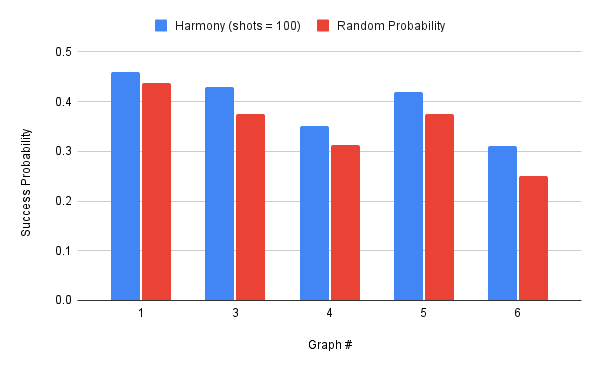
\includegraphics[width=.5\linewidth]{100shotGraph.png}
   \caption{$100$ shot}
   \label{fig:Harmony}
\end{figure} 

At 100 shots, GFPS has a higher probability of finding the maximal cut than by searching randomly. As the shot number increases to 500, this probability decreases and seems to converge with the random probability for graphs 5 and 6. However, neither of these experiments on harmony display significant increased success probability, that is to say, most advantage that the proposed oracle provides is destroyed by the noise present in NISQ devices.

\bigskip

\section{Simulation using small graph}
\label{sec:smallgraphs}



\bigskip

\section{Conclusion}
\label{sec:conclusion}



   %========================
   \bibliography{references}
   %========================

\end{document}